\documentclass{article}
\usepackage{graphicx}
\pagestyle{plain}

\oddsidemargin  -0.5 cm
\evensidemargin 0.0 cm
\textwidth      6.5in
\headheight     0.0in
\topmargin      -1 cm
\textheight=9.0in

\begin{document}
\Large

My biggest problem with the efficiency measurement was the
disagreement in number of tracks between data and MC.  One cut that
all events must pass through is ``number of tracks $\ge$ 3.''

To better understand what this would mean, I wanted to see what the
data distribution looks like below 3 tracks, which is technically hard
to do because only events which pass the {\bf hadron} cuts can be
found in pass2--- I can't, in general, loosen any cut.

So here's a work-around: the {\bf tau} subcollection is {\it
essentially} a superset of {\bf hadron}:
\begin{center}
  \includegraphics[width=\linewidth]{cuts.eps}
\end{center}
\begin{itemize}

  \item 2$^{\mbox{nd}}$ track p $<$ 85\% is very loose: for most
  hadrons, even the first track p is below a fifth of beam energy,

  \item cc-en(ergy) $<$ 85\% and big(est)-sh(ower) $<$ 85\% are
  numerically looser than the corresponding {\bf hadron} cuts, except
  that the {\bf hadron} versions of these cuts are not always applied.
  They are very highly correlated, though, as both of them are
  signatures of converted bhabhas,

  \item vis(ible)-en(ergy) $<$ 20\% is exactly the same, and

  \item n(umber of )tracks is looser in exactly the way I would want
  it to be, to see one more bin to the left.

\end{itemize}

From here on, I will assume that {\bf tau} is an exact superset of
{\bf hadron}.  (In an old notebook, I find that less than 1\% of the
events in {\bf hadron} fail {\bf tau}.  I can check the difference
more carefully later.)

\pagebreak
Here's the plot I wanted to see:
\begin{center}
  \vspace{-1 cm}
  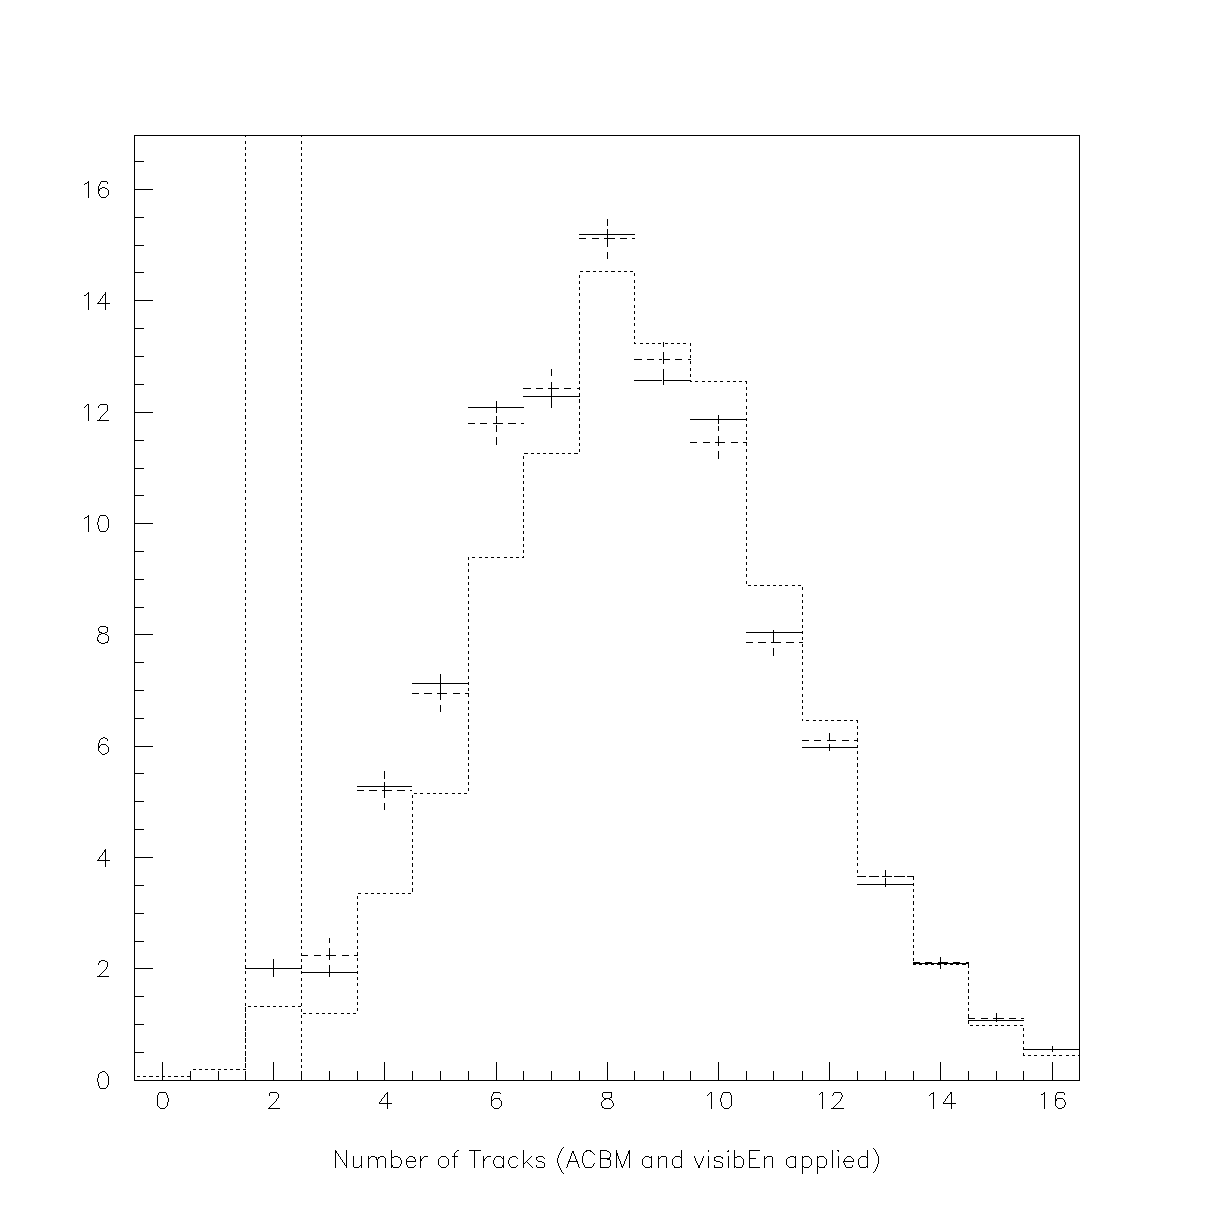
\includegraphics[width=\linewidth]{ntracks.eps}
\end{center}
\begin{itemize}

  \item The solid crosses are events from {\bf tau}, the dashed
  crosses are {\it some of the same events}, but from {\bf hadron},
  the dotted line is an infinite-statistics Monte Carlo sample.

  \item All {\bf hadron} cuts have been appplied except for ``number
  of tracks.''

  \item All are $\Upsilon(3S)$ and continuum-subtracted.  The {\bf
  hadron} histogram has been normalized to 100 (so that I can read
  percentages off the vertical axis).  (The appropriate scales for the
  other two histograms were found by applying all cuts so they are
  comparable, and then counting how many events were left in each.
  They {\it weren't} scaled by eye.)

\end{itemize}

\pagebreak
I would like to just read off this plot: ``after all other cuts in
{\bf hadron}, the number of tracks cut removes 2\% $\pm$few
$\Upsilon(3S)$ events.''  This assumes:
\begin{itemize}

  \item No data (that passes other cuts in {\bf hadron}) have 0 or 1
  tracks.  (I can't measure this without raw data.)

  \item The trigger is 100\% efficient for $e^+e^-$, $\mu^+\mu^-$, and
  $\tau^+\tau^-$ final states, as it is for hadrons.  (Of course it's
  not; the decay could have $\theta$ = 0.)

  \item The continuum subtraction removed all backgrounds.  The only
  one I would worry about is beamgas: after continuum subtraction,
  1.3\% of the remaining events are beamgas, and they tend to populate
  the low number-of-track bins.  (Before subtraction, contamination
  was 5\%--8\%, so the subtraction did some good!)

\end{itemize}
Here's what the same plot looks like with the least obtrusive beam-gas
cut:
\begin{center}
  \vspace{-1 cm}
  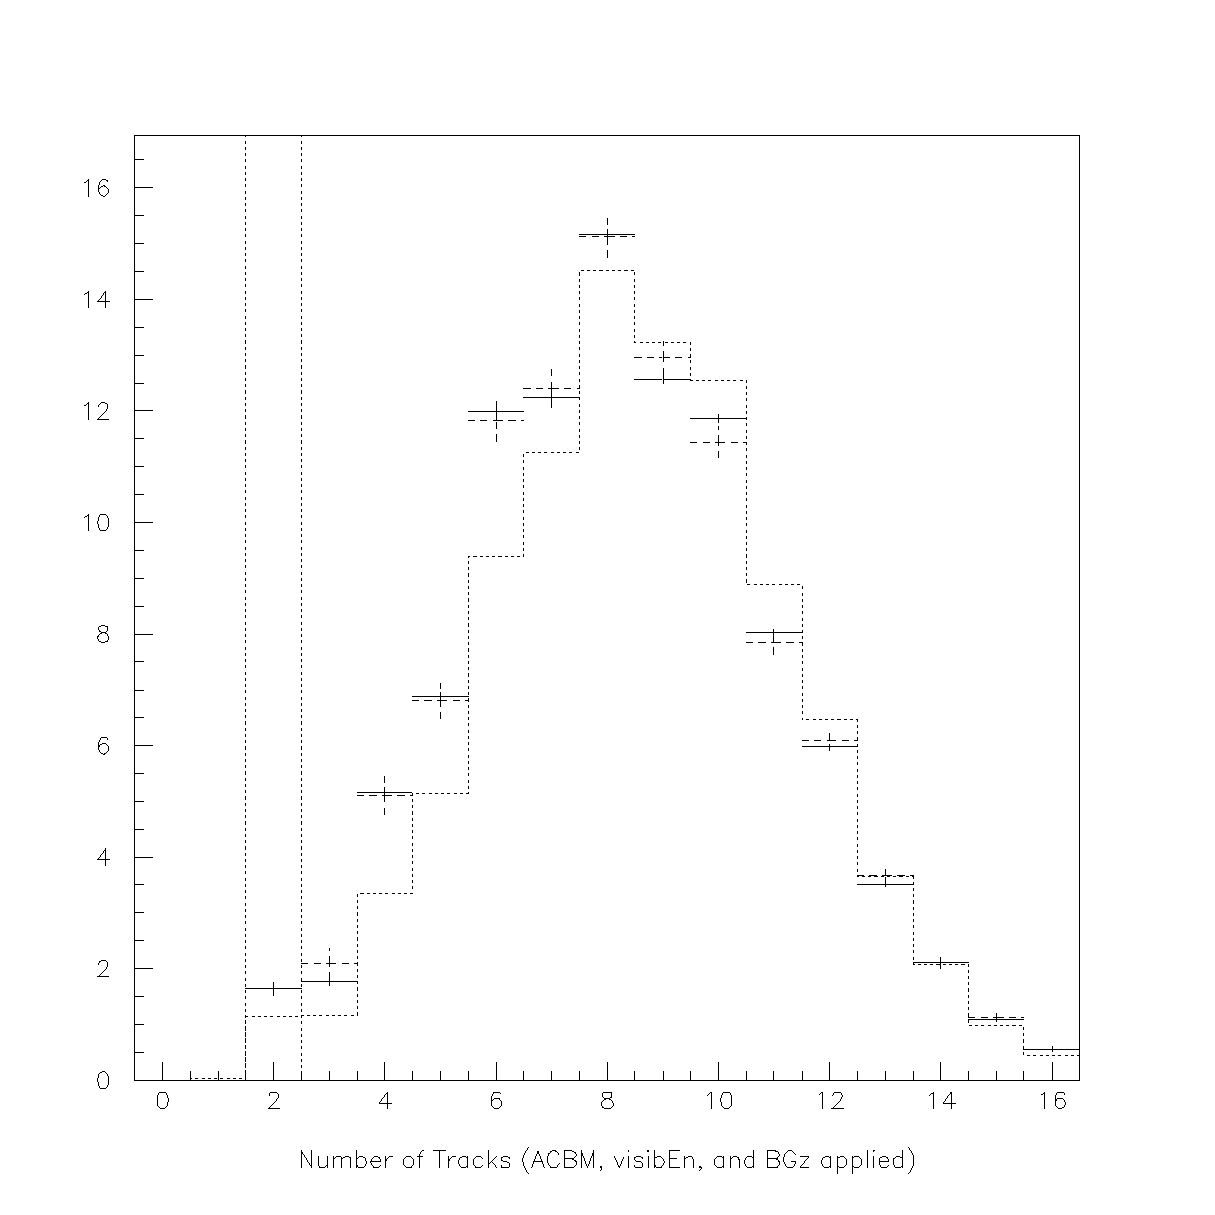
\includegraphics[width=0.8\linewidth]{ntracks_bgcut.eps}
\end{center}
(The beamgas cut shapes this plot beacuse two-track events don't form
a good vertex.  The $|z| <$ 5 cm cut is less obtrusive because the
distribution is dominated by beamspot size rather than tracking
resolution.

\pagebreak
\begin{center}
  \begin{tabular}{p{0.45\linewidth} p{0.45\linewidth}}
    \begin{minipage}{\linewidth}
      \Huge These are some other plots I made for myself.
    \end{minipage} &
    \begin{minipage}{\linewidth}
      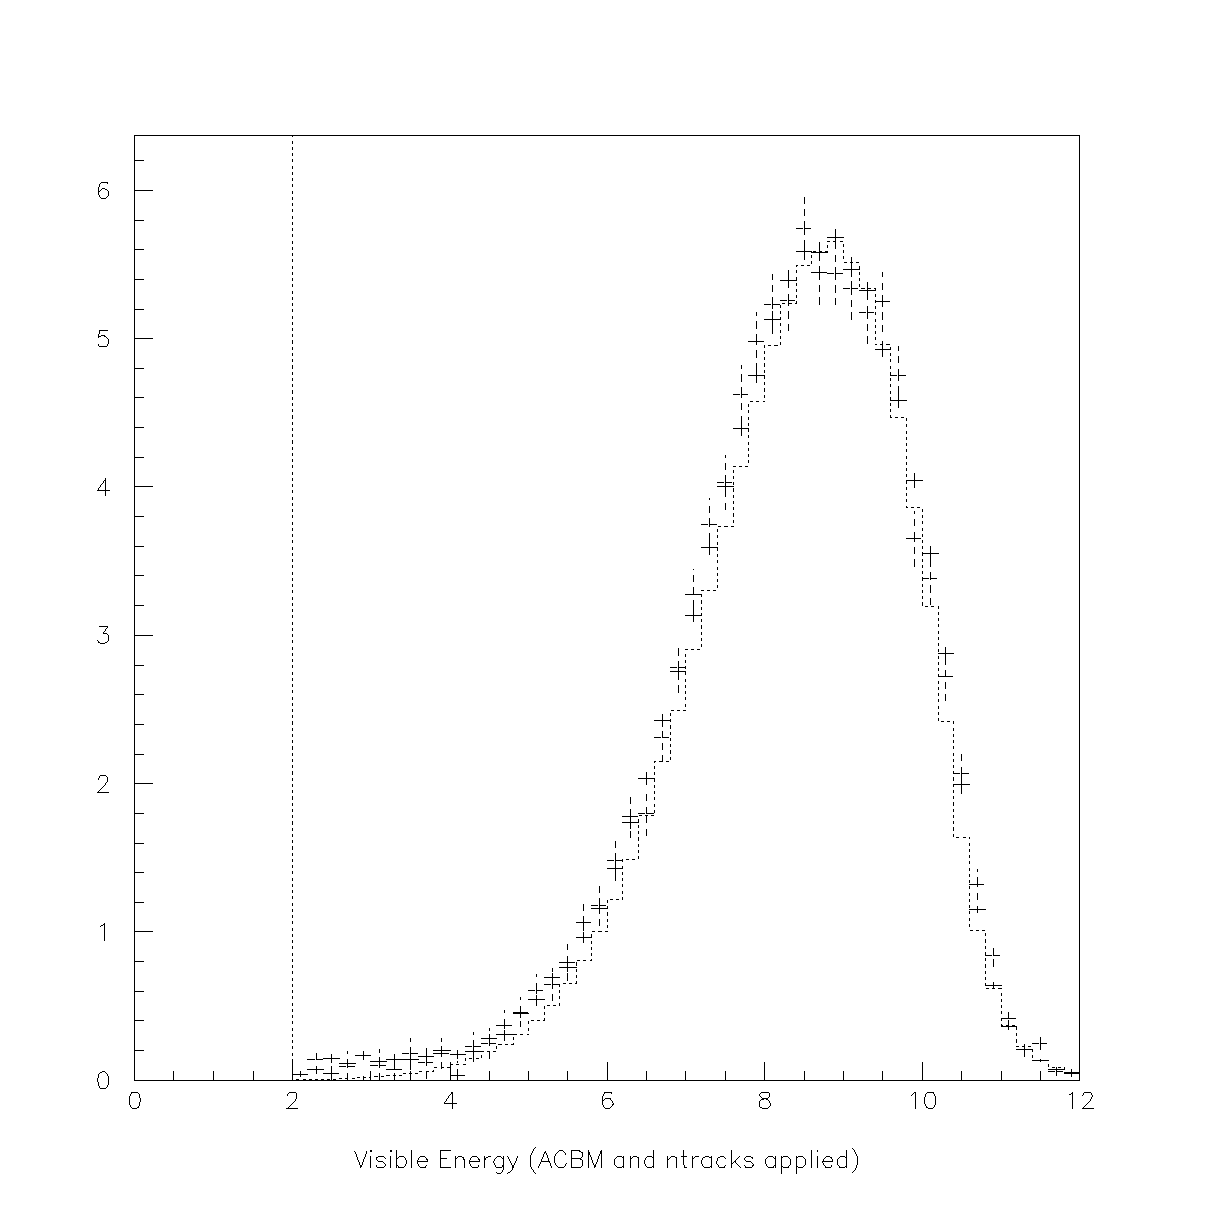
\includegraphics[width=\linewidth]{visiben.eps}
    \end{minipage} \\
    \begin{minipage}{\linewidth}
      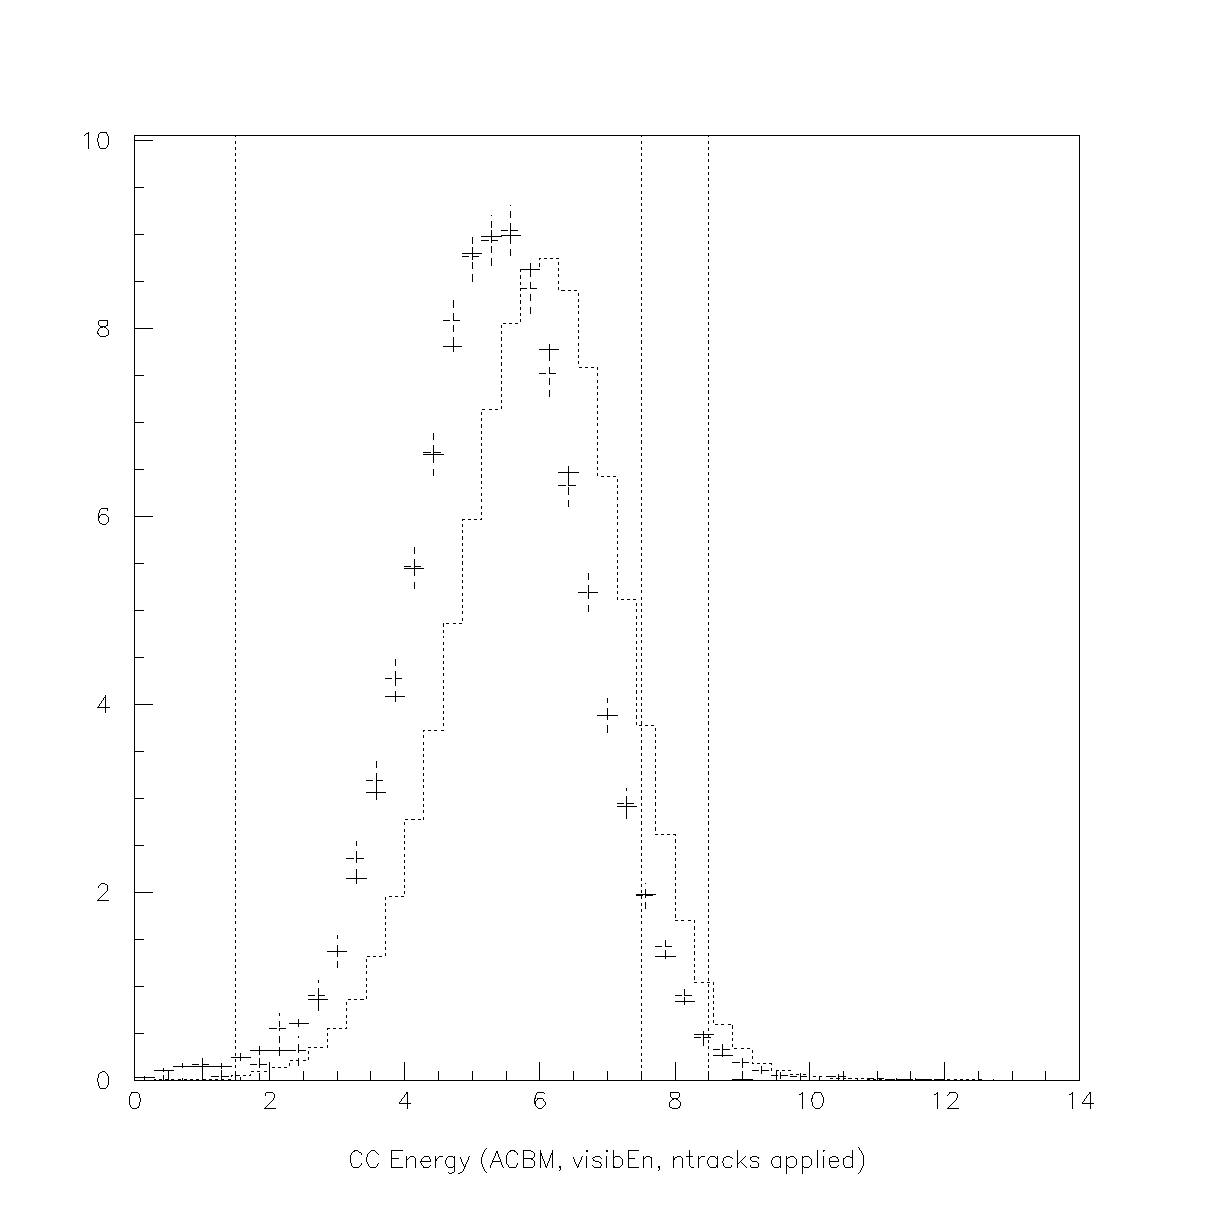
\includegraphics[width=\linewidth]{ccen.eps}
    \end{minipage} &
    \begin{minipage}{\linewidth}
      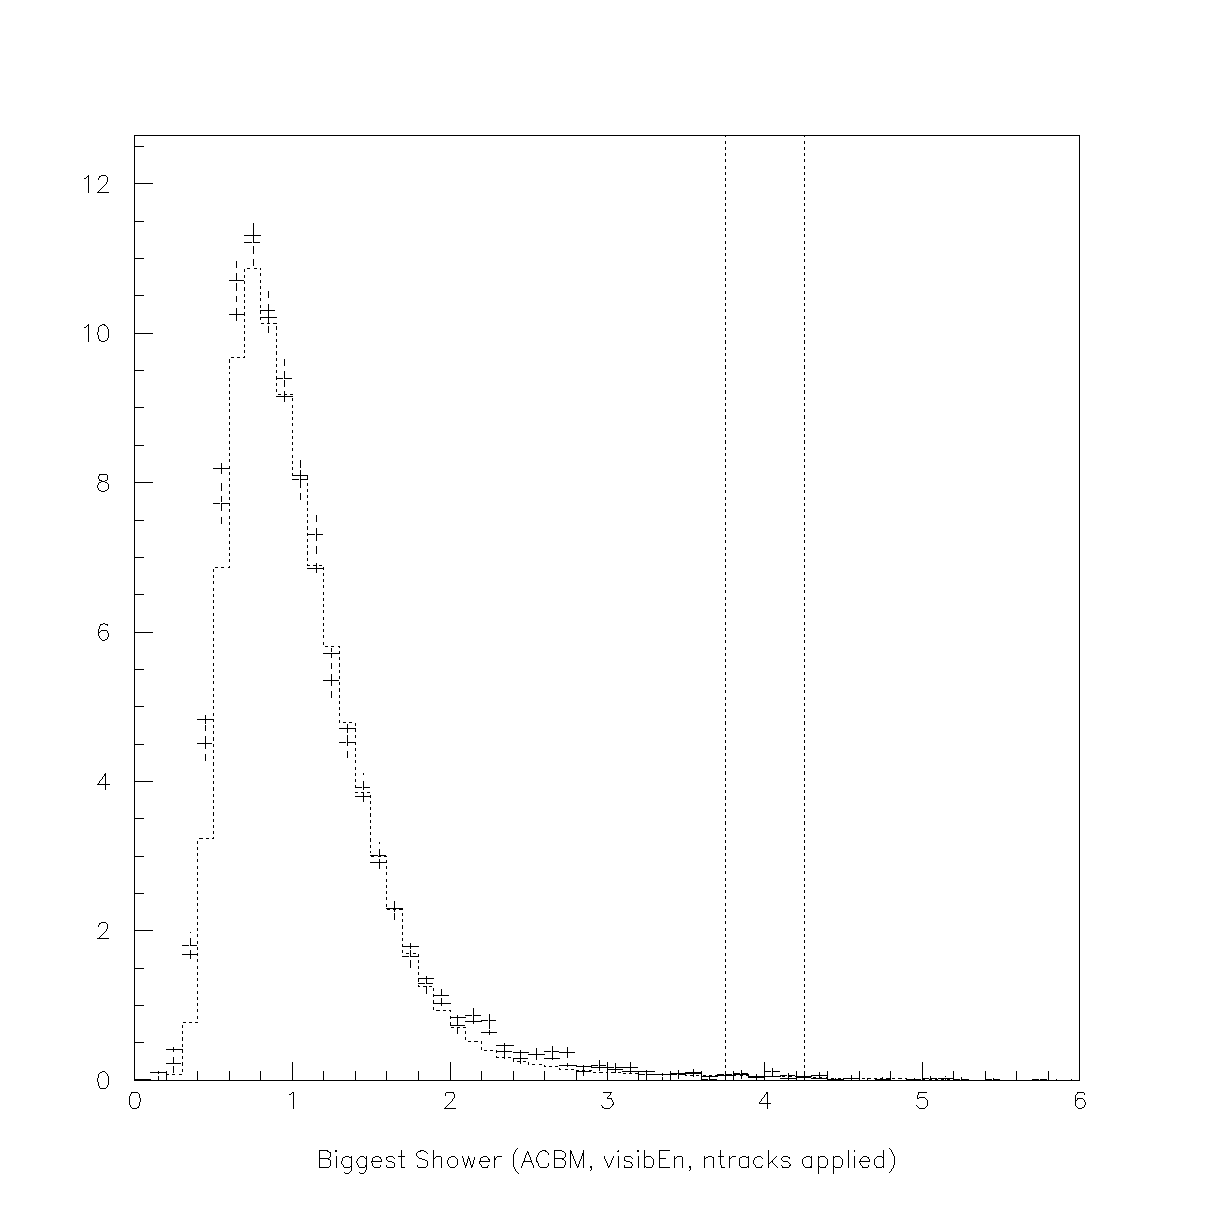
\includegraphics[width=\linewidth]{biggestsh.eps}
    \end{minipage}
  \end{tabular}
\end{center}

\vfill
{\Huge I just thought I would include everything.}
\vfill

\pagebreak
Having done this, I now have a better idea how to do the final
measurement:
\begin{enumerate}

  \item I will ask for about ninety runs of raw data: \{contniuum,
  peak, high-energy point\} $\otimes$ \{1S, 2S, 3S\} $\otimes$ about
  ten runs each, for precise continuum subtraction.  (I need the
  statistical error on the luminosity to be sub-percent.)

  These runs will be specially chosen for the beamgas to exactly
  cancel in the continuum subtraction, so that only $\Upsilon$ decays
  and cosmic rays would be left.

  \item Meanwhile, I will work with the Monte Carlo I now have to pick
  a set of cuts that exactly segregates $e^+e^-$, $\mu^+\mu^-$, and
  cosmic rays from other $\Upsilon$ decays.  My goal is to distinguish
  the two categories up to about 0.1\%, so that I can think about the
  other-$\Upsilon$ sample as being a pure and complete one.

  \item When I get the raw data, I will apply the cut and do a
  continuum subtraction so that I am left with only $\Upsilon \to
  \ldots \to$ hadron-or-tau.  The trigger efficiency for this is
  perfect (I need to find in my notebook the scientific-notation
  fraction of failures), so determining the efficiency would be a
  matter of applying the standard cuts and counting how many survive.

  \item If the cuts I choose in Monte Carlo are not perfect, I may
  need to assign a systematic error.  The beamgas count may also have
  an error, and, if I don't get as many runs as I want, the luminosity
  subtraction would introduce some error.

\end{enumerate}

This is better than a Monte Carlo cut-and-count because not only would
I be nearly independent of the Monte Carlo, but I wouldn't have to
break the efficiency measurement down mode-by-mode--- each of these
modes contributes to the uncertainty in efficiency.  (An analysis
which ignored all efficiency-related uncertainties {\it except} mode
measurement error had a total uncertainty of 0.7\%.)  It is especially
advantageous for the $\Upsilon(3S)$, which has about a hundred
different ways it can decay (counting ``$\to$ gluons/photon'' as a
single final state).

Having a lot of raw data runs on disk would also be very useful when
we start the luminosity measurement, since it would be just as
constraining to be bound to the {\bf bhabha} subcollection definition
as it was to be bound to {\bf hadron}.

\end{document}
